
\subsection*{Detailed Description}

\subsubsection*{Lobby}
When you have entered you identifiant, you arrive on the lobby page that have the name of the software \texttt{Sales Information System (SIS)}.

\begin{figure}[H]
  \centering
  
\includegraphics[width=0.4\textwidth]{./images/sis_lobby.png}
  \caption{Lobby of SIS}
  \label{fig:sis_lobby}
\end{figure}

\subsubsection*{Parties}
By clicking on \texttt{Parties} a new window appeared named \texttt{Maintain Parties}.

\begin{figure}[H]
  \centering
  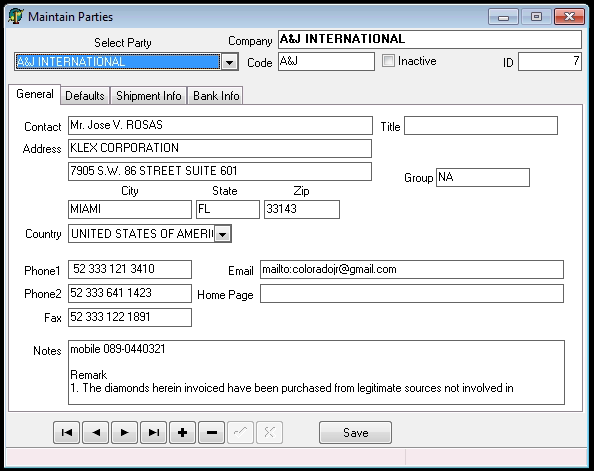
\includegraphics[width=0.4\textwidth]{./images/sis_parties_general.png}
  \caption{Maintain Parties window}
  \label{fig:sis_parties_general}
\end{figure}

The window is here to manage the parties database (or client).

\paragraph*{Top of the page}
By clicking on the down arrow below \texttt{Select Party}, a drop-down menu appeared.

\begin{figure}[H]
  \centering
  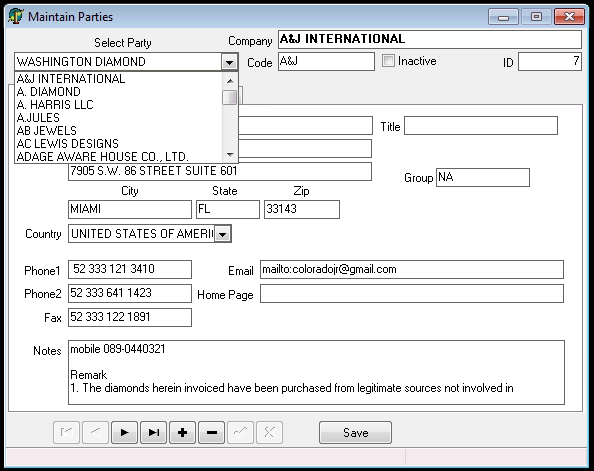
\includegraphics[width=0.4\textwidth]{./images/sis_parties_selectparty.png}
  \caption{Select Party drop-down}
  \label{fig:sis_parties_selectparty}
\end{figure}

Here you have all the already record parties in lexicographical order.

Then the general fields are written :
\begin{itemize}
  \item \texttt{Company} name of the company
  \item \texttt{Code} its identifier code, will be written on the series number of products
  \item \texttt{ID} identifier key in the database
  \item \texttt{Inactive} (bool) by default is False
\end{itemize}

Those fields are the required fields needed for having an instance of Party and so for its creation.

The following fields are nullable.

\paragraph*{General}
By clicking on \texttt{General} (default view) you have a view of the general information (Contact, Address, etc).

\begin{figure}[H]
  \centering
  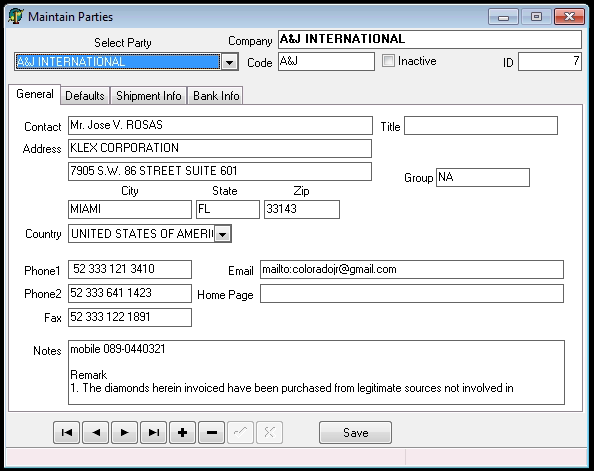
\includegraphics[width=0.4\textwidth]{./images/sis_parties_general.png}
  \caption{General tab of Maintain Parties}
  \label{fig:sis_parties_general_tab}
\end{figure}

You can edit those fields here : Contact, Title, Address (Country, City, State, Zip), Groups, Phone, email, fax, home page and notes.

\paragraph*{Defaults}
By clicking on \texttt{Defaults} the following view is displayed.

\begin{figure}[H]
  \centering
  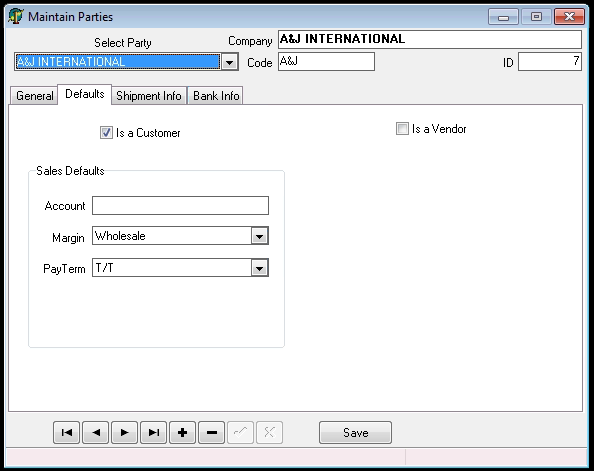
\includegraphics[width=0.4\textwidth]{./images/sis_parties_defaults.png}
  \caption{Defaults tab of Maintain Parties}
  \label{fig:sis_parties_defaults}
\end{figure}

If you tick \texttt{Is a Vendor}, it display more options.

You can edit those fields here : Account, Margin, PayTerm.

\begin{figure}[H]
  \centering
  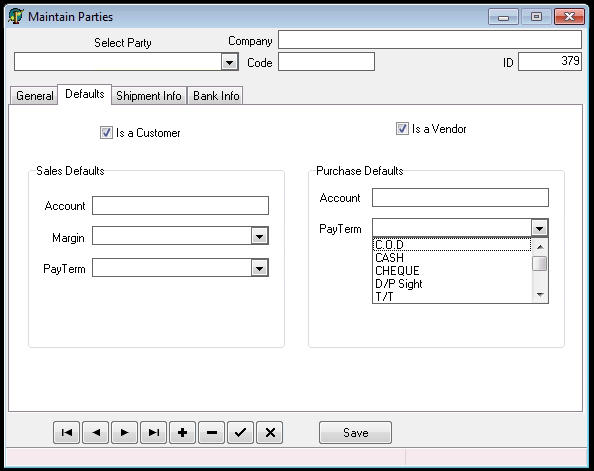
\includegraphics[width=0.4\textwidth]{./images/sis_parties_defaults_vendor.png}
  \caption{Defaults (Vendor) tab of Maintain Parties}
  \label{fig:sis_parties_defaults_vendor}
\end{figure}

The drop-down menu \texttt{Margin} contains the one that are managed on \texttt{PDP}.

Remarks :
\begin{itemize}
  \item Account is generally empty

    If find only two parties that contains it 
    \begin{itemize}
      \item Kemeya : BKK Feb 12
      \item Tank : 18\%
    \end{itemize}

  \item The \texttt{Vendor} is generally not used. Only two occurrences found :
    \begin{itemize}
      \item Lenovre Jewelery
      \item TC
    \end{itemize}

  So those fields are considered useless.
\end{itemize}

\paragraph*{Shipment Info}
By clicking on \texttt{Shipment Info} the following view is displayed.

\begin{figure}[H]
  \centering
  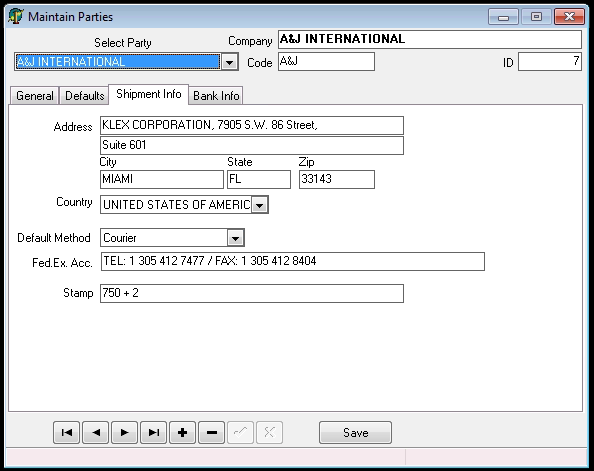
\includegraphics[width=0.4\textwidth]{./images/sis_parties_shipmentinfo.png}
  \caption{Shipment Info tab of Maintain Parties}
  \label{fig:sis_parties_shipmentinfo}
\end{figure}

You can edit those fields here : Address (Country, City, State, Zip), Default Method, Fed.\ Ex.\ Acc.\ and Stamp.

\paragraph*{Bank Info}
By clicking on \texttt{Bank Info} the following view is displayed.

\begin{figure}[H]
  \centering
  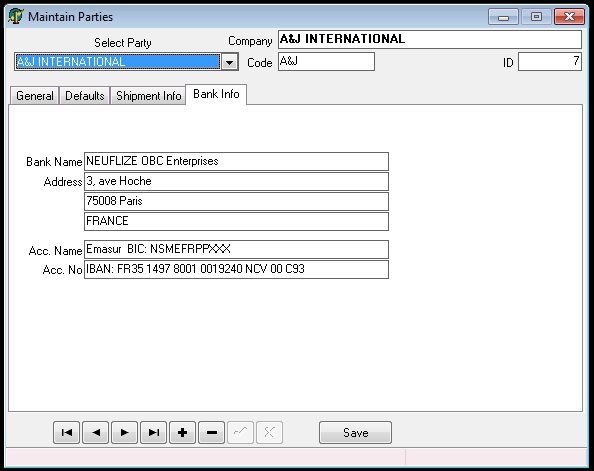
\includegraphics[width=0.4\textwidth]{./images/sis_parties_bankinfo.png}
  \caption{Bank Info tab of Maintain Parties}
  \label{fig:sis_parties_bankinfo}
\end{figure}

You can edit those fields here : Bank Name, Address, Acc.\ Name, Acc.\ No.

\paragraph*{New}
By clicking on \texttt{+}, display an empty Party.

\begin{figure}[H]
  \centering
  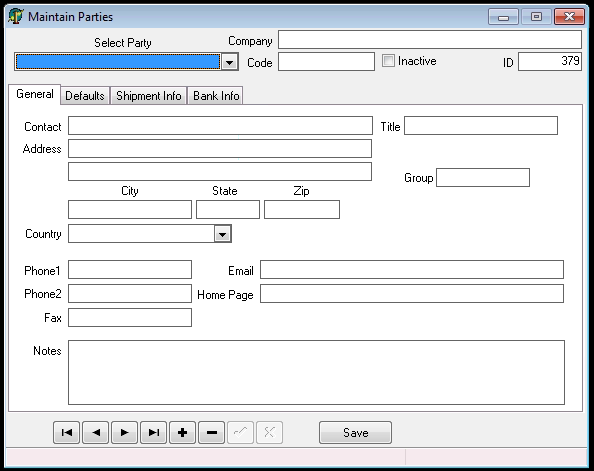
\includegraphics[width=0.4\textwidth]{./images/sis_parties_new_general.png}
  \caption{New Party blank form}
  \label{fig:sis_parties_new_blank}
\end{figure}

From here in \texttt{Defaults}, \texttt{Shipment Info} and \texttt{Bank Info} are blank in the same way as \texttt{General}.

The \texttt{ID} field have been automatically created. It seems to increment of one for each party created.

For adding a new party you have to fill the general field at the top first \texttt{Company} and \texttt{Code}. \texttt{Inactive} is by default on \emph{False}.

Then you can click on \texttt{Save} to create the instance.

If you do not do it SIS will send an error.

\begin{figure}[H]
  \centering
  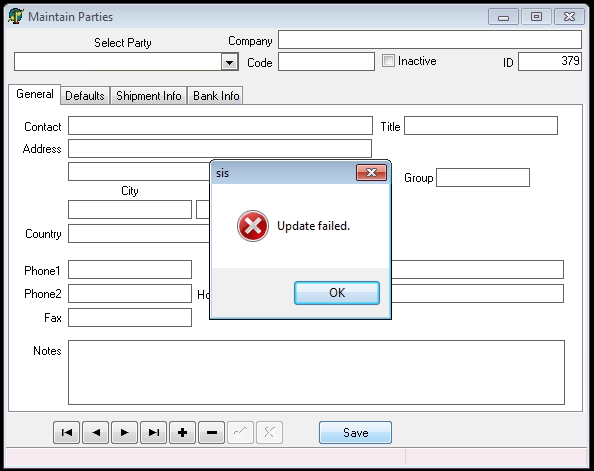
\includegraphics[width=0.4\textwidth]{./images/sis_parties_errorupdatefailed.png}
  \caption{Error when required general field is empty}
  \label{fig:sis_parties_error}
\end{figure}

This error will also be sent if you empty one of the general fields on an existing instance.

\subsubsection*{Quotations, Book Orders and Shipment Goods}
Those pages are quite similar. We will call the general format a \texttt{Document Manager} window.

By clicking on \texttt{Quotations} you arrive on \texttt{Maintain Sales Quotations}, this is used with new client or client where there is a possibility of \texttt{Cancellation}.

\begin{figure}[H]
  \centering
  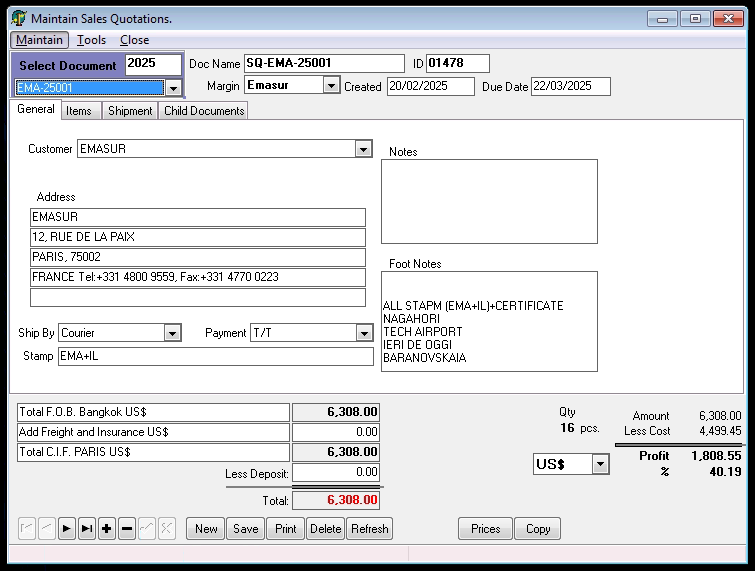
\includegraphics[width=0.4\textwidth]{./images/sis_quotations_general.png}
  \caption{Maintain Sales Quotations window}
  \label{fig:sis_quotations_general}
\end{figure}

By clicking on \texttt{Book Orders} you arrive on \texttt{Maintain Sales Orders}, this is used to manage and create \textbf{Sales Orders}.

\begin{figure}[H]
  \centering
  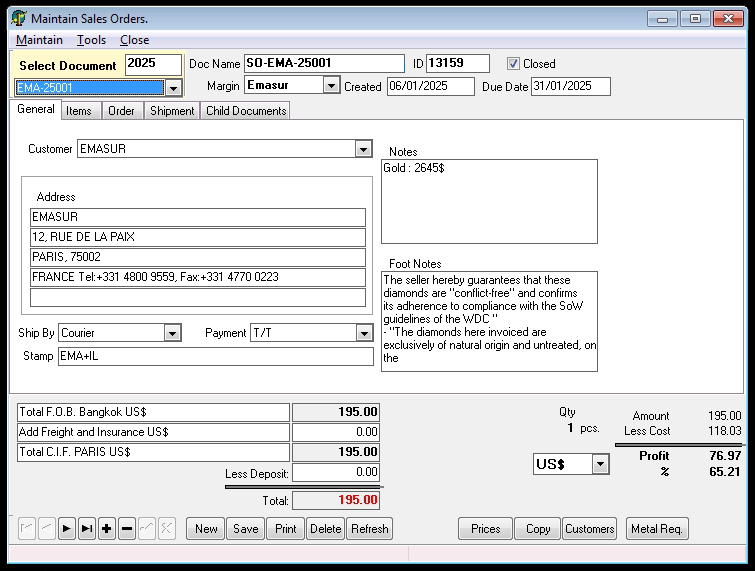
\includegraphics[width=0.4\textwidth]{./images/sis_orders_general.png}
  \caption{Maintain Sales Orders window}
  \label{fig:sis_orders_general}
\end{figure}

By clicking on \texttt{Shipment Goods} you arrive on \texttt{Maintain Sales Invoices}, this is used to manage and create \textbf{Invoices}.

\begin{figure}[H]
  \centering
  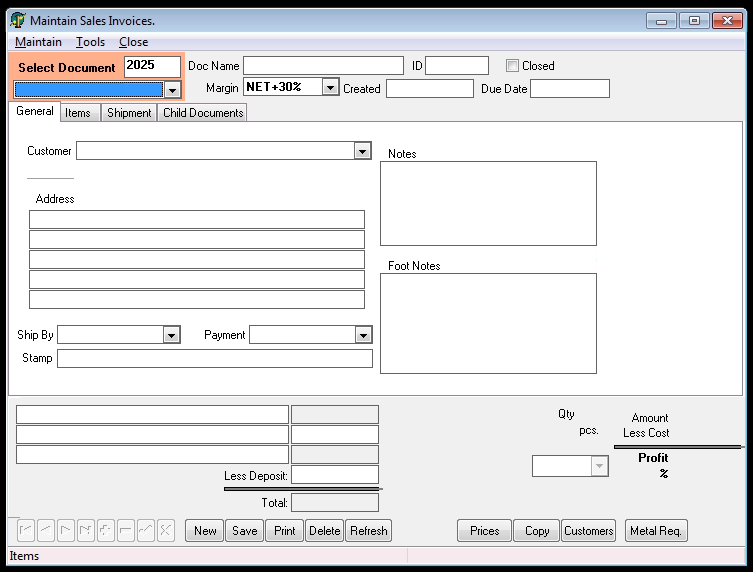
\includegraphics[width=0.4\textwidth]{./images/sis_invoices_default.png}
  \caption{Maintain Sales Invoices window}
  \label{fig:sis_invoices_default}
\end{figure}

Here you can see that they are almost exactly the same. In \texttt{Orders} you can find one more option, the menu \texttt{Order}. So we will focus on the \texttt{Sales Orders} pages.

\paragraph*{Required Field}
On the top of the page you can find the required fields.
\begin{itemize}
  \item \texttt{Doc Name} name of the document
  \item \texttt{ID} identifier in the database
  \item \texttt{Closed} boolean
  \item \texttt{Margin} choices one of the margins managed in PDP
  \item \texttt{Created} date of creation
  \item \texttt{Due Date} date of the expecting result (delivery limit for example)
\end{itemize}

\paragraph*{General}
By clicking on \texttt{General} (open by default), the following view is displayed.

\begin{figure}[H]
  \centering
  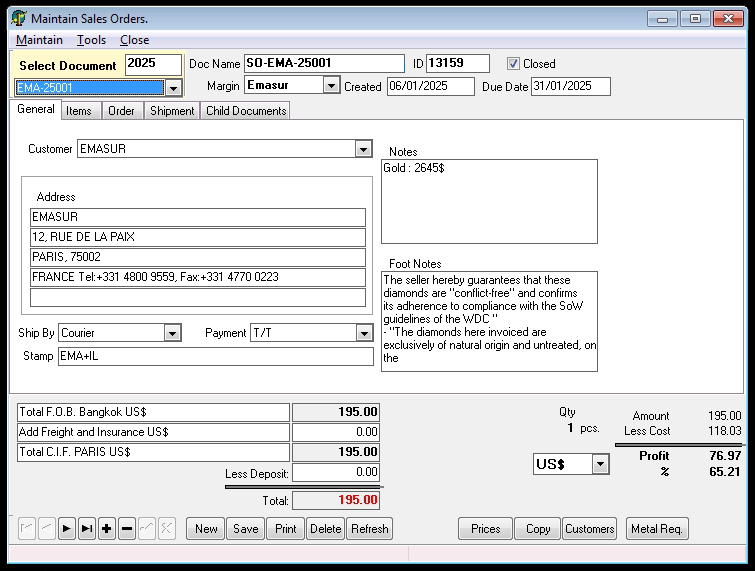
\includegraphics[width=0.4\textwidth]{./images/sis_orders_general.png}
  \caption{General tab of Sales Orders}
  \label{fig:sis_orders_general_tab}
\end{figure}

You can edit those fields here : Customer, Address, Ship By, Payment, Stamp, Notes, Foot notes.

\paragraph*{Items/General}
By clicking on \texttt{Items/General}, the following view is displayed. By default the \texttt{General} sub-menu has opened.

\begin{figure}[H]
  \centering
  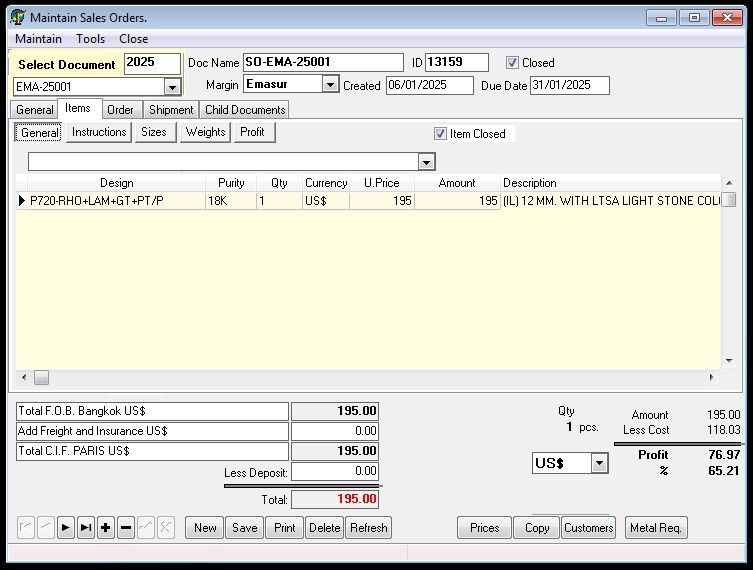
\includegraphics[width=0.4\textwidth]{./images/sis_orders_items_general.png}
  \caption{Items/General sub-tab of Sales Orders}
  \label{fig:sis_orders_items_general}
\end{figure}

It contains a table with these fields:
\begin{itemize}
  \item \textbf{Design} (\texttt{MODEL-COLORS/M})
  \item \textbf{Purity}
  \item \textbf{Qty}
  \item \textbf{Currency}
  \item \textbf{U.Price}
  \item \textbf{Amount}
  \item \textbf{Description}
\end{itemize}

You can find the references of the products ordered by the customer with multiple informations.

\paragraph*{Items/Instructions}
By clicking on \texttt{Items/Instructions}, the following view is displayed. By default the \texttt{Instructions} sub-menu has opened.

\begin{figure}[H]
  \centering
  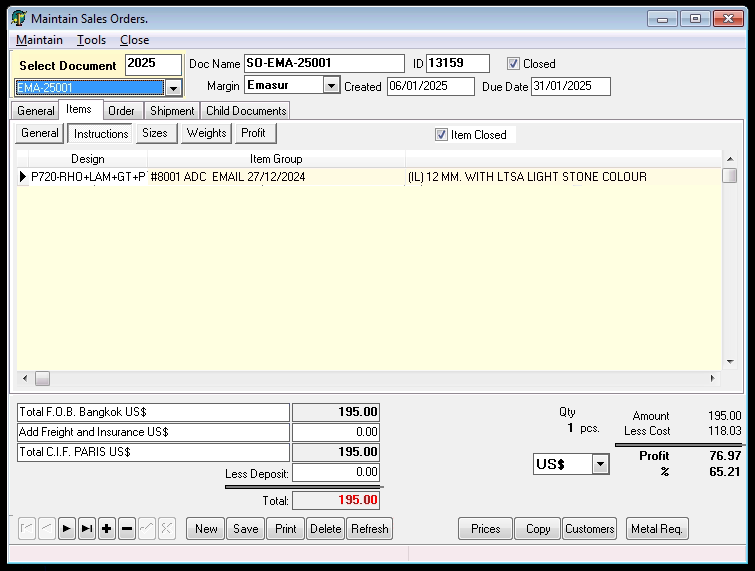
\includegraphics[width=0.4\textwidth]{./images/sis_orders_items_instructions.png}
  \caption{Items/Instructions sub-tab of Sales Orders}
  \label{fig:sis_orders_items_instructions}
\end{figure}

It contains a table with these fields:
\begin{itemize}
  \item \textbf{Design} (\texttt{MODEL-COLORS/M})
  \item \textbf{Item Group}
  \item \textbf{Special Instruction}
\end{itemize}

You can find the references of the products ordered by the customer with the fields \texttt{Item Group} and \texttt{Special Instruction}.

\paragraph*{Items/Sizes}
By clicking on \texttt{Items/Sizes}, the following view is displayed. By default the \texttt{Sizes} sub-menu has opened.

\begin{figure}[H]
  \centering
  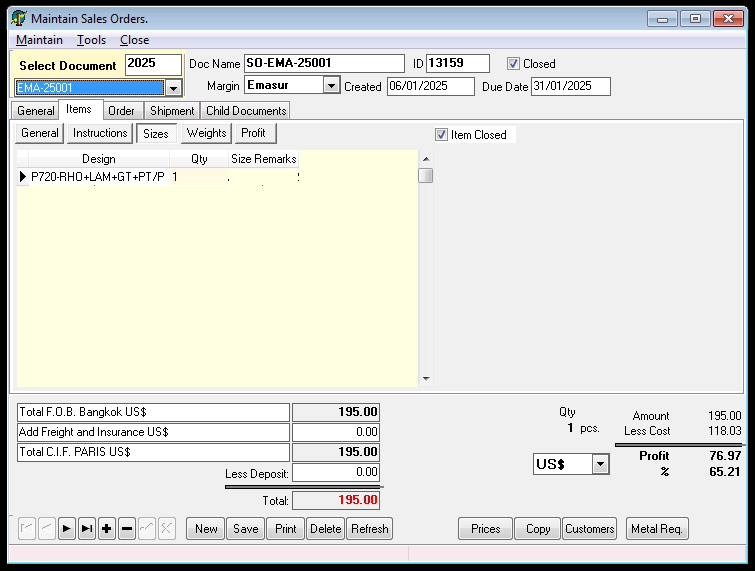
\includegraphics[width=0.4\textwidth]{./images/sis_orders_items_sizes.png}
  \caption{Items/Sizes sub-tab of Sales Orders}
  \label{fig:sis_orders_items_sizes}
\end{figure}

It contains a table with these fields:
\begin{itemize}
  \item \textbf{Design} (\texttt{MODEL-COLORS/M})
  \item \textbf{Qty}
  \item \textbf{Size Remarks}
\end{itemize}

You can find the references of the products ordered by the customer with the fields \texttt{Qty} and \texttt{Size Remarks}.

\paragraph*{Items/Weights}
By clicking on \texttt{Items/Weights}, the following view is displayed. By default the \texttt{Weights} sub-menu has opened.

\begin{figure}[H]
  \centering
  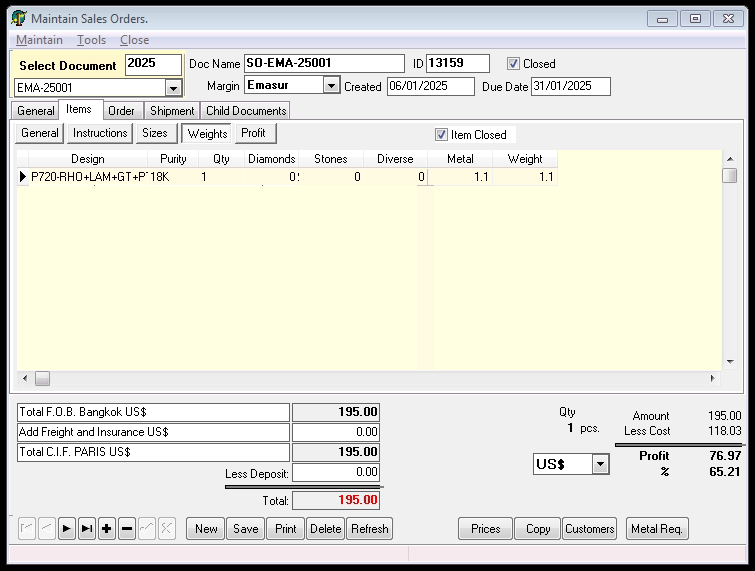
\includegraphics[width=0.4\textwidth]{./images/sis_orders_items_weights.png}
  \caption{Items/Weights sub-tab of Sales Orders}
  \label{fig:sis_orders_items_weights}
\end{figure}

It contains a table with these fields:
\begin{itemize}
  \item \textbf{Design} (\texttt{MODEL-COLORS/M})
  \item \textbf{Purity}
  \item \textbf{Qty}
  \item \textbf{Diamonds}
  \item \textbf{Stones}
  \item \textbf{Diverse}
  \item \textbf{Metal}
  \item \textbf{Weight}
\end{itemize}

You can find the references of the products ordered by the customer with fields that detail the weight.

\paragraph*{Items/Profit}
By clicking on \texttt{Items/Profit}, the following view is displayed. By default the \texttt{Profit} sub-menu has opened.

\begin{figure}[H]
  \centering
  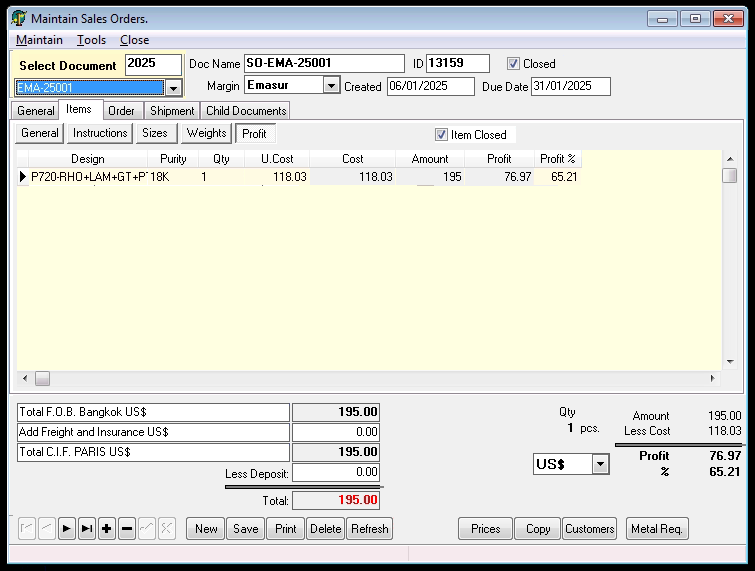
\includegraphics[width=0.4\textwidth]{./images/sis_orders_items_profit.png}
  \caption{Items/Profit sub-tab of Sales Orders}
  \label{fig:sis_orders_items_profit}
\end{figure}

It contains a table with these fields:
\begin{itemize}
  \item \textbf{Design} (\texttt{MODEL-COLORS/M})
  \item \textbf{Purity}
  \item \textbf{Qty}
  \item \textbf{U. Cost}
  \item \textbf{Cost}
  \item \textbf{Amount}
  \item \textbf{Profit}
  \item \textbf{Profit \%}
\end{itemize}

This table details the profit calculation by reference.

\paragraph*{Order}
By clicking on \texttt{Order}, the following view is displayed.

\begin{figure}[H]
  \centering
  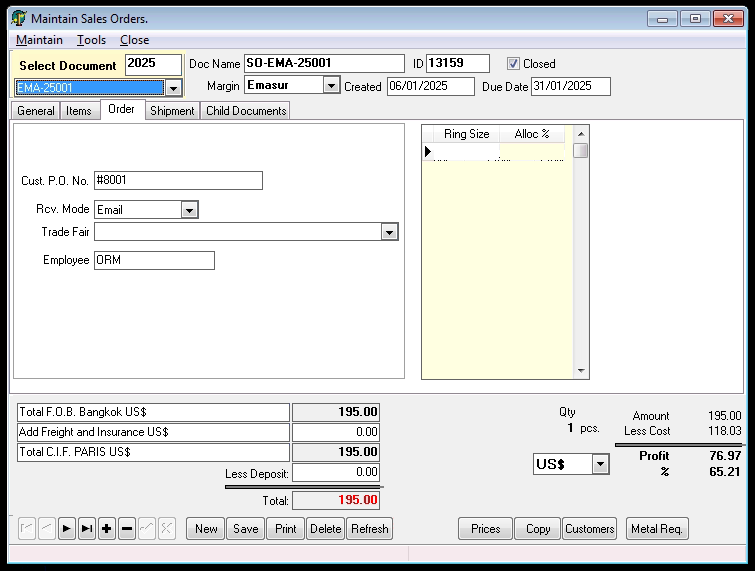
\includegraphics[width=0.4\textwidth]{./images/sis_orders_order.png}
  \caption{Order tab of Sales Orders}
  \label{fig:sis_orders_order}
\end{figure}

You can edit those fields here:
\begin{itemize}
  \item \texttt{Cust P.O. No.} stands for \emph{Customer Purchase Order Number}, this is the reference number from the client.
  \item \texttt{Rcv, Mode} stands for \emph{Receiving Mode}.
  \item \texttt{Trade Fair} is used if the order was made during one.
  \item \texttt{Employee} contains the name of the employee responsible for this order.
\end{itemize}

\paragraph*{Shipment}
By clicking on \texttt{Shipment}, the following view is displayed.

\begin{figure}[H]
  \centering
  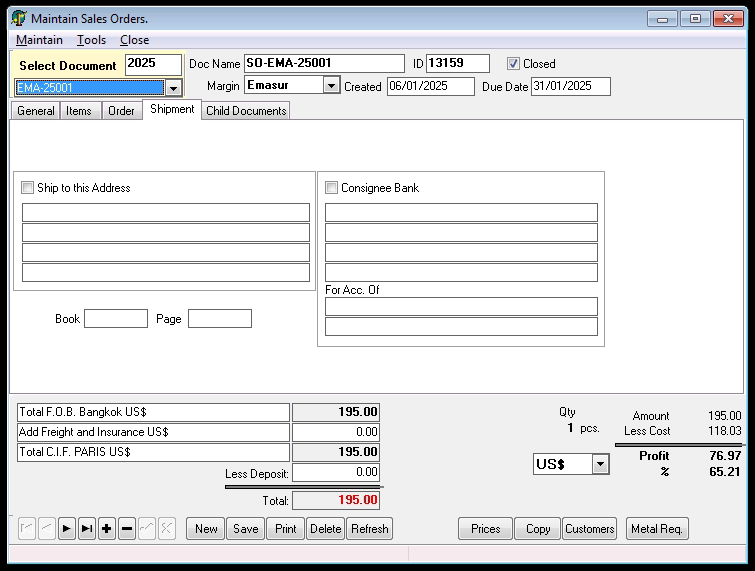
\includegraphics[width=0.4\textwidth]{./images/sis_orders_shipment.png}
  \caption{Shipment tab of Sales Orders}
  \label{fig:sis_orders_shipment}
\end{figure}

You can edit those fields here: Ship to this Address (bool), Consignee Bank (bool), For Acc.\ Of, Book, Page

If needed, you can specify delivery details here.

\paragraph*{Child Documents}
By clicking on \texttt{Child Documents}, the following view is displayed.

\begin{figure}[H]
  \centering
  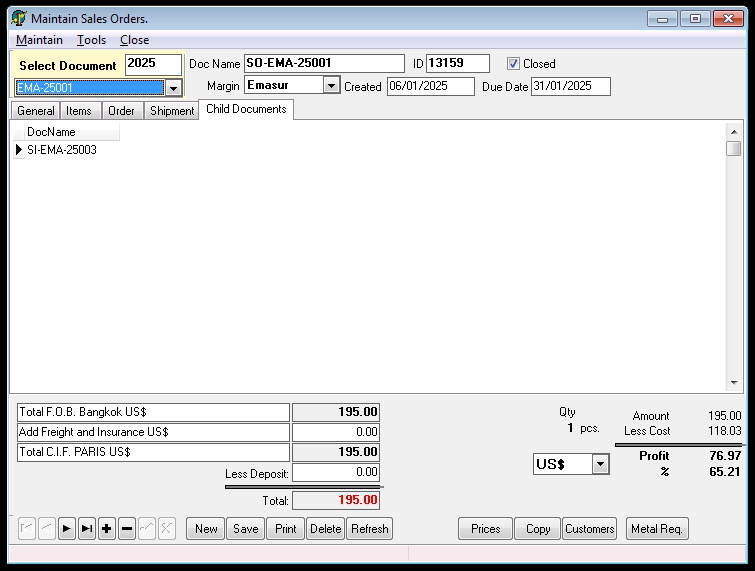
\includegraphics[width=0.4\textwidth]{./images/sis_orders_childdocuments.png}
  \caption{Child Documents tab of Sales Orders}
  \label{fig:sis_orders_childdocuments}
\end{figure}

It contains a table with only one field \texttt{DocName} (\texttt{DOCTYPE-AAA-XXXXX}).

List \texttt{Document} that come from the current one. In this case we have a sale order \texttt{SO-EMA-250001} which has been sent through the sale invoice \texttt{SI-EMA-250003}.

It can happen that multiple invoices are used for one order. And then on one invoice it contains product from different sales orders.

\paragraph*{Profit Details}
At the bottom of the page you have the details of the profit.

\begin{figure}[H]
  \centering
  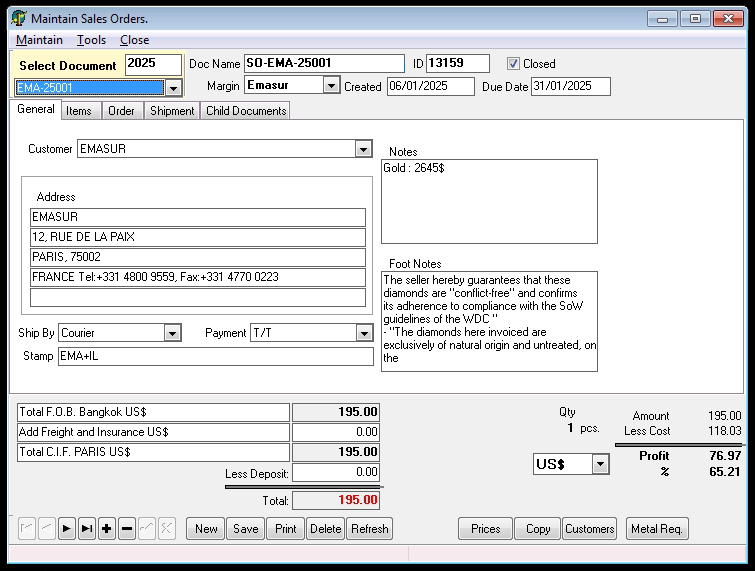
\includegraphics[width=0.4\textwidth]{./images/sis_orders_general.png}
  \caption{Profit Details at bottom of Sales Orders (reused screenshot)}
  \label{fig:sis_orders_profit_details}
\end{figure}

It contains those fields that are computed automatically.
\begin{itemize}
  \item Total F.O.B Bangkok US\$
  \item Add Freight and Insurance US\$
  \item Total C.I.F PARIS US\$
  \item Less Deposit
  \item Total
\end{itemize}

Finally on the right you can specify the currency with a drop-down menu.  
And another table shows:
\begin{itemize}
  \item Qty
  \item Amount
  \item Less Cost
  \item Profit
  \item Profit in \%
\end{itemize}

\paragraph*{New}
By clicking on \texttt{New} at the bottom of the page, a new instance of a sale is created.

\begin{figure}[H]
  \centering
  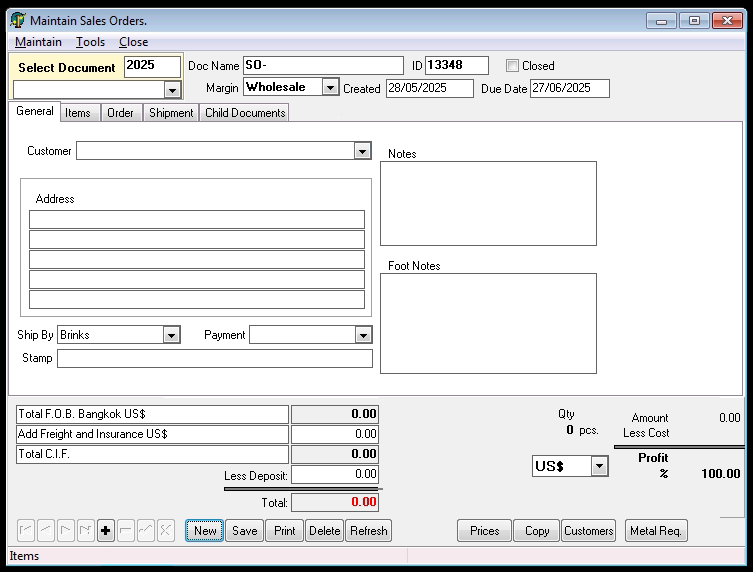
\includegraphics[width=0.4\textwidth]{./images/sis_orders_new.png}
  \caption{New Sales Order form}
  \label{fig:sis_orders_new}
\end{figure}

All the fields \texttt{Items}, \texttt{Order}, \texttt{Shipment} and \texttt{Child Documents} are empty like \texttt{General}.

We can notice that \textbf{by default} the document type is indicated:
\begin{itemize}
  \item \texttt{Doc Name} :
    \begin{itemize}
      \item \texttt{SQ-} for \texttt{Quotations}
      \item \texttt{SO-} for \texttt{Sales Order}
      \item \texttt{SI-} for \texttt{Sales Invoice}
    \end{itemize}
  \item \texttt{ID} : automatically created by incrementing from the last one
  \item \texttt{Closed} : False by default
  \item \texttt{Margin} : \texttt{Wholesale}
  \item \texttt{Created} : the current date
  \item \texttt{Due Date} : One month after the current date
\end{itemize}

\paragraph*{Print}
By clicking on \texttt{Print} at the bottom of the page, the window \texttt{Print Document} will be displayed.

\begin{figure}[H]
  \centering
  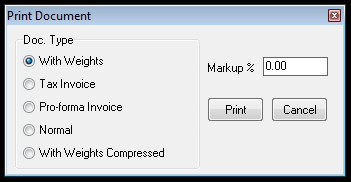
\includegraphics[width=0.4\textwidth]{./images/sis_orders_print.png}
  \caption{Print Document window}
  \label{fig:sis_orders_print}
\end{figure}

Here we can notice:
\begin{itemize}
  \item \texttt{With Weights} : Print the sales orders/quotations with the weights details
\end{itemize}

Remarks:
\begin{itemize}
  \item Actually only the \texttt{With Weights} format is used.
\end{itemize}

\paragraph*{Prices}
By clicking on \texttt{Prices} at the bottom of the page, the window \texttt{Product Prices} will be displayed.

\begin{figure}[H]
  \centering
  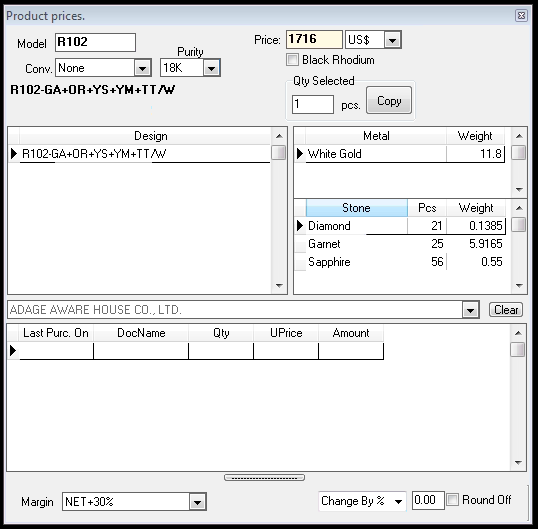
\includegraphics[width=0.4\textwidth]{./images/sis_orders_prices.png}
  \caption{Product Prices window}
  \label{fig:sis_orders_prices}
\end{figure}

Here you can indicate:
\begin{itemize}
  \item Model
  \item Conv (other metal than white gold)
  \item Purity
  \item Qty
  \item Select a design
\end{itemize}
It will give you on two tables details on the product: one table with Metal, Weight and the other with Stone, Pcs, Weight.  
Then you have at the top the field \texttt{Price} that indicates the price; you can also choose the currency with a drop-down menu.

A table at the bottom seems to refer to similar orders. It contains these fields:
\begin{itemize}
  \item Last Purc.\ On
  \item DocName
  \item Qty
  \item Uprice
  \item Amount
\end{itemize}

And a drop-down menu allows you to select a specific customer.

On this window you can search in the database managed by PDP the model and references of products. It allows you to indicate the appropriate prices for each item.

\paragraph*{Copy}
By clicking on \texttt{Copy} at the bottom of the page, the window \texttt{Document Browser} will be displayed.

\begin{figure}[H]
  \centering
  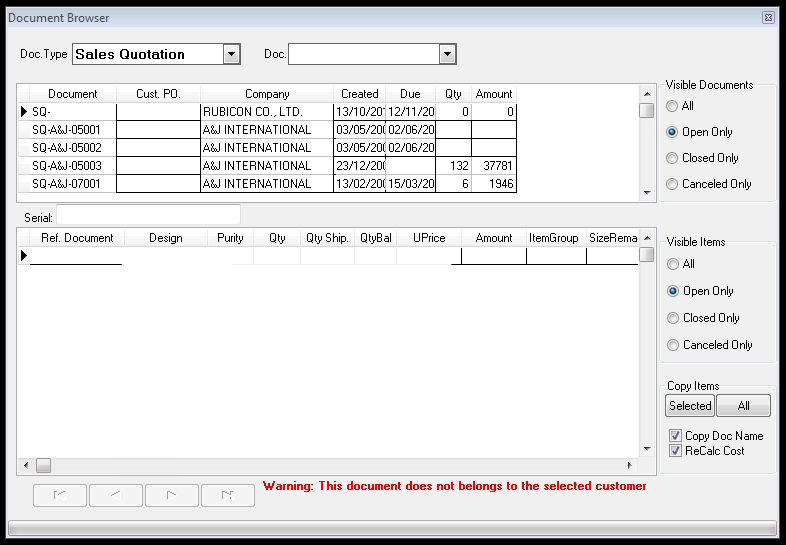
\includegraphics[width=0.4\textwidth]{./images/sis_orders_copy.png}
  \caption{Document Browser window}
  \label{fig:sis_orders_copy}
\end{figure}

Here you can filter by \texttt{Doc.\ Types} and \texttt{Doc.} with a drop-down menu and by their boolean attribute: \texttt{Open}, \texttt{Closed}, \texttt{Canceled} with tick boxes.

Then, in the table below it, the documents appear with these fields:
\begin{itemize}
  \item \textbf{Document} (\texttt{DOCTYPE-AAA-XXXXX})
  \item \textbf{Cust.\ PO.} (empty here)
  \item \textbf{Company}
  \item \textbf{Created} (date)
  \item \textbf{Due} (date)
  \item \textbf{Qty}
  \item \textbf{Amount}
\end{itemize}

Then a second table where you can filter with the field \texttt{Serial} contains these fields:
\begin{itemize}
  \item \textbf{Ref.\ Document}
  \item \textbf{Design}
  \item \textbf{Purity}
  \item \textbf{Qty}
  \item \textbf{Qty Ship.}
  \item \textbf{QtyBal}
  \item \textbf{Uprice}
  \item \textbf{Amount}
  \item \textbf{ItemGroup}
  \item \textbf{SizeRemarks}
  \item \dots
\end{itemize}

This window allows you to copy \texttt{Item} from other \texttt{Document} of any kind.  
Because you are on \texttt{Sales Orders} it looks at \texttt{Sales Quotation} by default.

\paragraph*{Customers}
By clicking on \texttt{Customers} at the bottom of the page, the window \texttt{Maintain Parties} will be displayed.

\begin{figure}[H]
  \centering
  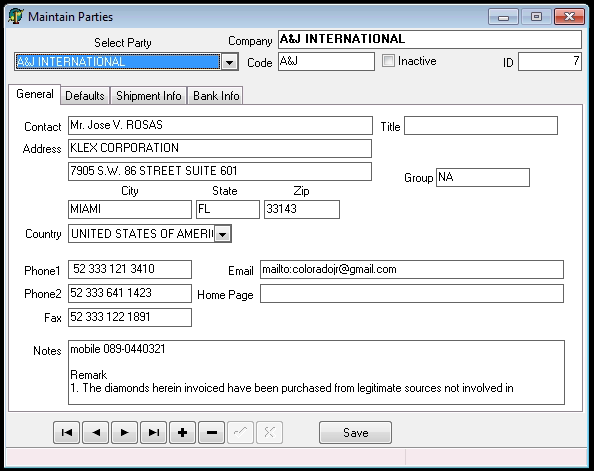
\includegraphics[width=0.4\textwidth]{./images/sis_parties_general.png}
  \caption{Maintain Parties window (reused)}
  \label{fig:sis_parties_general_reuse}
\end{figure}

\paragraph*{Metal Weight Summary}
By clicking on \texttt{Metal Req.} at the bottom of the page, the window \texttt{Metal Weight Summary} will be displayed.

\begin{figure}[H]
  \centering
  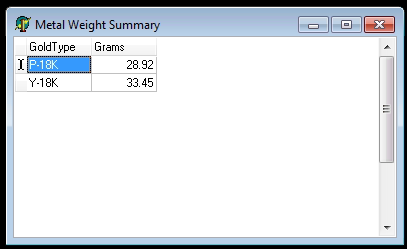
\includegraphics[width=0.4\textwidth]{./images/sis_orders_metal_req.png}
  \caption{Metal Weight Summary window}
  \label{fig:sis_orders_metal_req}
\end{figure}

It contains a table with two fields:
\begin{itemize}
  \item \textbf{GoldType} (\texttt{M-PURITY})
  \item \textbf{Grams}
\end{itemize}

\paragraph*{Toolbar Maintain}
By clicking on \texttt{Maintain} you have a drop-down menu that appeared.

\begin{figure}[H]
  \centering
  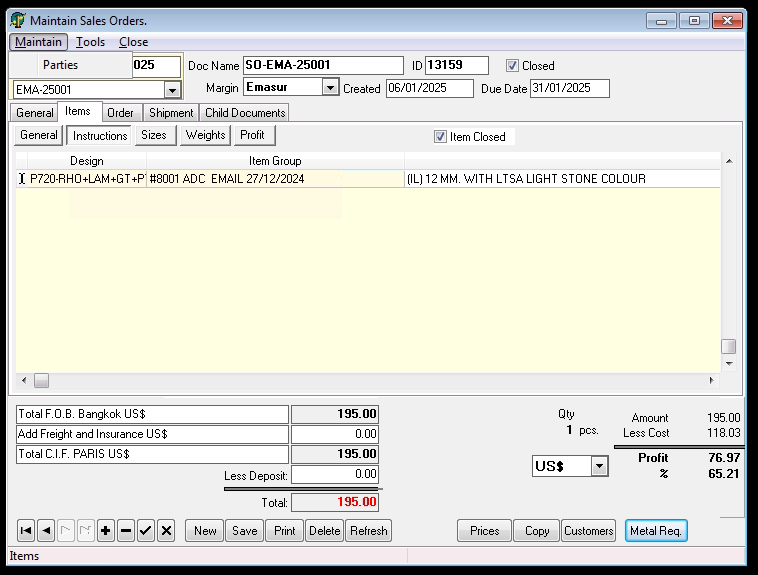
\includegraphics[width=0.4\textwidth]{./images/sis_orders_maintain.png}
  \caption{Toolbar Maintain menu}
  \label{fig:sis_orders_maintain}
\end{figure}

With only \texttt{Parties} that will open the \texttt{Maintain Parties} window seen before.

\paragraph*{Toolbar Tools}
By clicking on \texttt{Tools} you have a drop-down menu that appeared.

\begin{figure}[H]
  \centering
  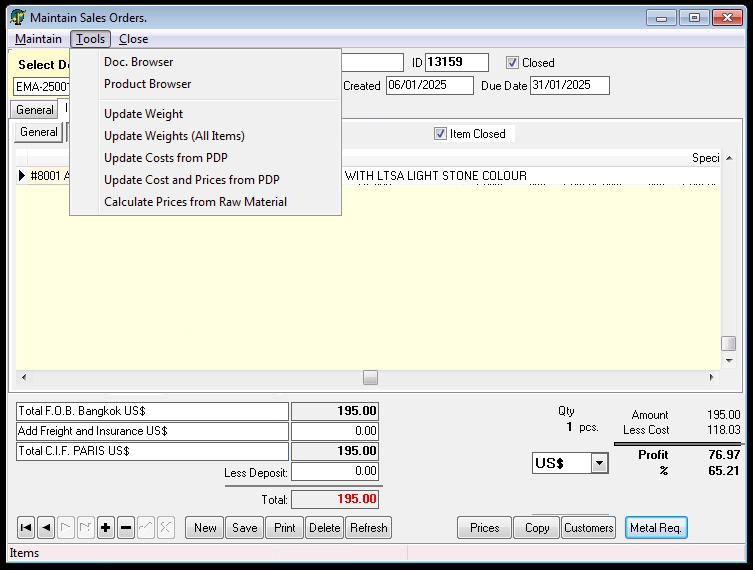
\includegraphics[width=0.4\textwidth]{./images/sis_orders_tools.png}
  \caption{Toolbar Tools menu}
  \label{fig:sis_orders_tools}
\end{figure}

It contains these options:
\begin{itemize}
  \item Doc.\ Browser : open the \texttt{Document Browser} window
  \item Product Browser : open the \texttt{Product Prices} window as seen later
  \item Update Weight
  \item Update Weights (All Items)
  \item Update Costs from PDP
  \item Update Cost and Prices from PDP
  \item Calculate Prices from Raw Material
\end{itemize}

All the ones that start with \texttt{Update} will check if changes occurred in the database and will refresh accordingly the data.

Finally, by clicking on \texttt{Calculate Prices from Raw Material}, the window \texttt{Update Price from Raw-Material} is displayed.

\begin{figure}[H]
  \centering
  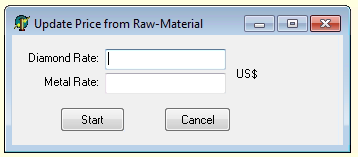
\includegraphics[width=0.4\textwidth]{./images/sis_orders_tools_updatepricefromraw.png}
  \caption{Update Price from Raw-Material window}
  \label{fig:sis_orders_tools_updatepricefromraw}
\end{figure}

Here you can fill two fields:
\begin{itemize}
  \item Diamond Rate
  \item Metal Rate
\end{itemize}
Then there are two buttons \texttt{Start} and \texttt{Cancel}.

\subsubsection*{Lobby Application}
On the toolbar, if you click on \texttt{Application} a drop-down menu appeared.

\begin{figure}[H]
  \centering
  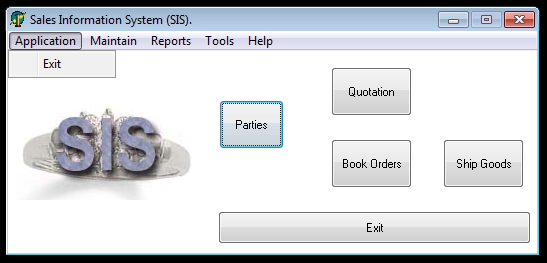
\includegraphics[width=0.4\textwidth]{./images/sis_lobby_application.png}
  \caption{Lobby Application menu}
  \label{fig:sis_lobby_application}
\end{figure}

Here you have an \texttt{Exit} button.

\subsubsection*{Lobby Maintain}
On the toolbar, if you click on \texttt{Maintains} a drop-down menu appeared.

\begin{figure}[H]
  \centering
  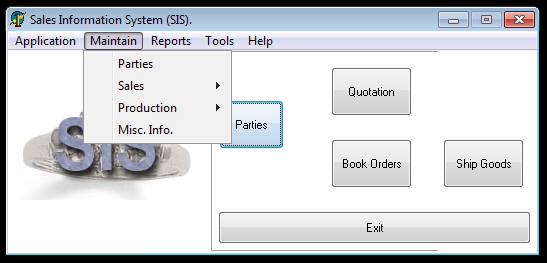
\includegraphics[width=0.4\textwidth]{./images/sis_lobby_maintain.png}
  \caption{Lobby Maintain menu}
  \label{fig:sis_lobby_maintain}
\end{figure}

It contains those options:
\begin{itemize}
  \item Parties
  \item Sales
  \item Production
  \item Misc.\ Info.
\end{itemize}

\paragraph*{Parties}
\texttt{Parties} will open the \texttt{Maintain Parties} window.

\paragraph*{Sales}
Clicking on \texttt{Sales} will display other possibilities on the drop-down menu.

\begin{figure}[H]
  \centering
  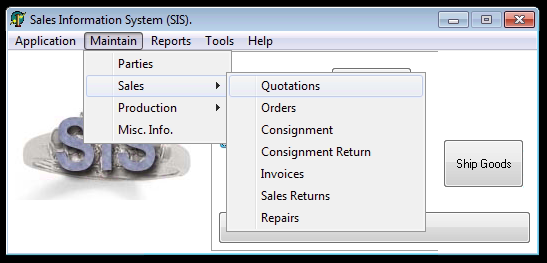
\includegraphics[width=0.4\textwidth]{./images/sis_lobby_maintain_sales.png}
  \caption{Lobby Maintain \texttt{Sales} menu}
  \label{fig:sis_lobby_maintain_sales}
\end{figure}

\begin{itemize}
  \item Quotations
  \item Orders
  \item Consignment
  \item Consignment Return
  \item Invoices
  \item Sales Returns
  \item Repairs
\end{itemize}

All those sales documents have been seen earlier or have more or less the same format as \texttt{Quotations}, etc. They are other \texttt{Document Types} but less common.

\paragraph*{Production}
Clicking on \texttt{Production} will display other possibilities.

\begin{figure}[H]
  \centering
  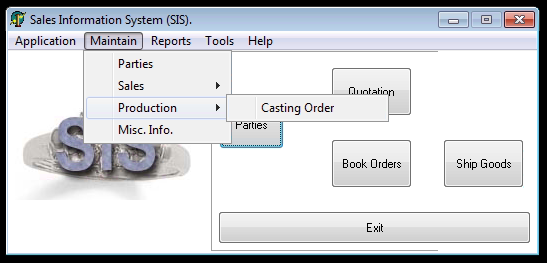
\includegraphics[width=0.4\textwidth]{./images/sis_lobby_maintain_production.png}
  \caption{Lobby Maintain \texttt{Production} menu}
  \label{fig:sis_lobby_maintain_production}
\end{figure}

Which is also a \texttt{Document Manager} window but its goal is unclear.

\paragraph*{Misc.\ Info.}
Clicking on \texttt{Misc.\ Info.} will open the window \texttt{Miscellaneous Information}.  
This window manages multiple tables of general information. You can edit those informations and save them by clicking on \texttt{Save} at the bottom-right of the page.

\subparagraph*{Business Areas}

\begin{figure}[H]
  \centering
  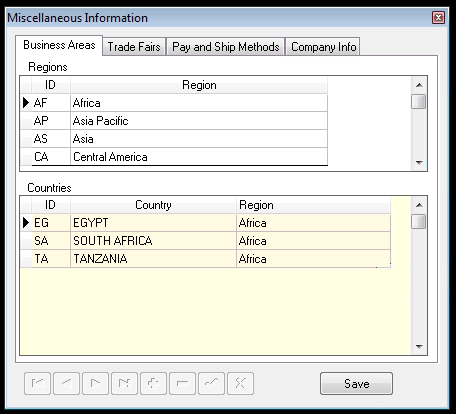
\includegraphics[width=0.4\textwidth]{./images/sis_lobby_maintain_miscinfo_businessareas.png}
  \caption{Business Areas sub-window of Misc.\ Info.}
  \label{fig:sis_lobby_maintain_miscinfo_businessareas}
\end{figure}

Such as:
\begin{itemize}
  \item \texttt{Region} : ID , Region
  \item \texttt{Country}: ID, Country, Region
\end{itemize}

\subparagraph*{Trade Fairs}

\begin{figure}[H]
  \centering
  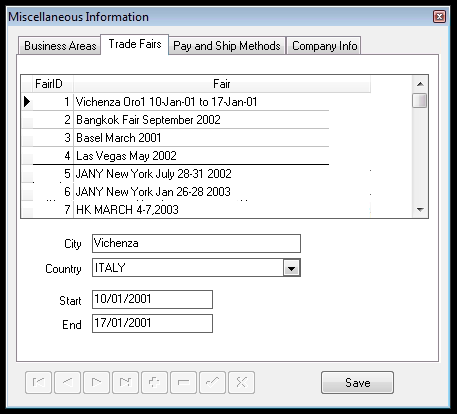
\includegraphics[width=0.4\textwidth]{./images/sis_lobby_maintain_miscinfo_tradefairs.png}
  \caption{Trade Fairs sub-window of Misc.\ Info.}
  \label{fig:sis_lobby_maintain_miscinfo_tradefairs}
\end{figure}

That contains, for each \texttt{Fair}:
\begin{itemize}
  \item FairID
  \item Fair
  \item City
  \item Country
  \item Start (date)
  \item End (date)
\end{itemize}

\subparagraph*{Pay and Ship Methods}

\begin{figure}[H]
  \centering
  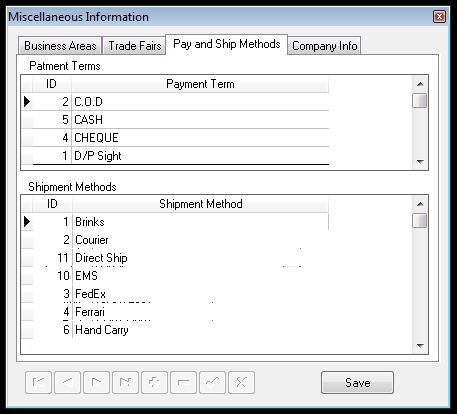
\includegraphics[width=0.4\textwidth]{./images/sis_lobby_maintain_miscinfo_payandshipmethods.png}
  \caption{Pay and Ship Methods sub-window of Misc.\ Info.}
  \label{fig:sis_lobby_maintain_miscinfo_payandshipmethods}
\end{figure}

That contains two tables:
\begin{itemize}
  \item \texttt{Payment Terms} (certainly payment terms) : ID, Payment Term
  \item \texttt{Shipment Methods} : ID, Shipment Method
\end{itemize}

\subparagraph*{Company Info}

\begin{figure}[H]
  \centering
  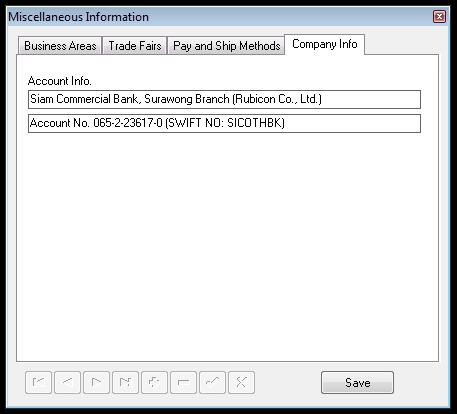
\includegraphics[width=0.4\textwidth]{./images/sis_lobby_maintain_miscinfo_companyinfo.png}
  \caption{Company Info sub-window of Misc.\ Info.}
  \label{fig:sis_lobby_maintain_miscinfo_companyinfo}
\end{figure}

With two fields named \texttt{Account Info.}.

\subsubsection*{Lobby Reports}
On the toolbar, if you click on \texttt{Reports} a drop-down menu appeared.

\begin{figure}[H]
  \centering
  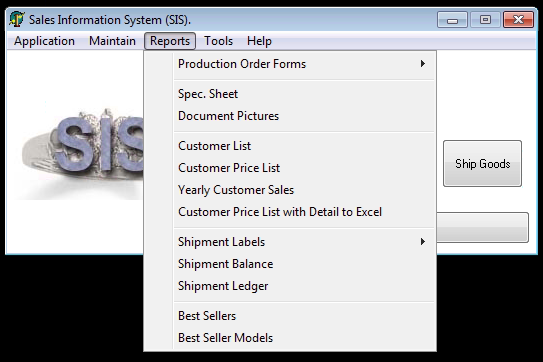
\includegraphics[width=0.4\textwidth]{./images/sis_lobby_reports.png}
  \caption{Lobby Reports menu}
  \label{fig:sis_lobby_reports}
\end{figure}

It contains these options:
\begin{itemize}
  \item Production Order Forms
  \item Spec.\ Sheet
  \item Document Pictures
  \item Customer List
  \item Customer Price List
  \item Yearly Customer Sales
  \item Customer Price List with Detail to Excel
  \item Shipment Labels
  \item Shipment Balance
  \item Shipment Ledger
  \item Best Sellers
  \item Best Sellers Model
\end{itemize}

\paragraph*{Production Order Forms}
By clicking on \texttt{Production Order Forms} other possibilities are displayed.

\begin{figure}[H]
  \centering
  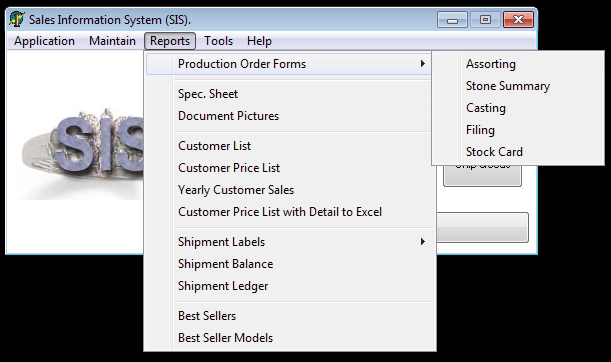
\includegraphics[width=0.4\textwidth]{./images/sis_lobby_reports_productionorderforms.png}
  \caption{Production Order Forms sub-menu}
  \label{fig:sis_lobby_reports_productionorderforms}
\end{figure}

\begin{itemize}
  \item Assorting
  \item Stone Summary
  \item Casting
  \item Filling
  \item Stock Card
\end{itemize}

\paragraph*{Shipment Labels}
By clicking on \texttt{Shipment Labels} other possibilities are displayed.

\begin{figure}[H]
  \centering
  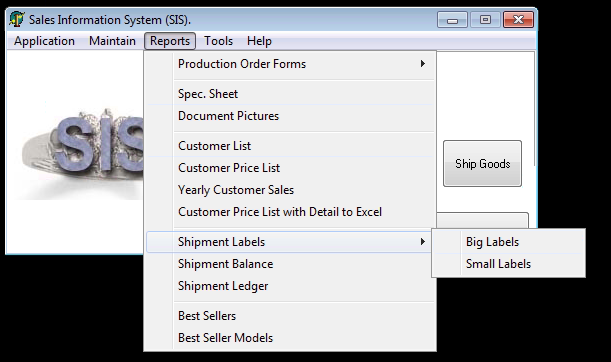
\includegraphics[width=0.4\textwidth]{./images/sis_lobby_reports_shipmentlabels.png}
  \caption{Shipment Labels sub-menu}
  \label{fig:sis_lobby_reports_shipmentlabels}
\end{figure}

\begin{itemize}
  \item Big Labels
  \item Small Labels
\end{itemize}

\paragraph*{Report}
All of the options that are in this menu allow you to create an appropriate report.

Clicking on one of these options will either generate the report directly or display the \texttt{Parameters} window.

\begin{figure}[H]
  \centering
  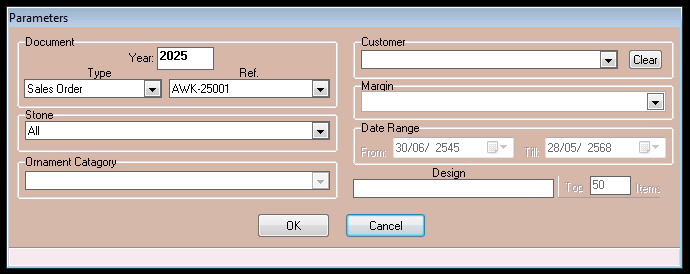
\includegraphics[width=0.4\textwidth]{./images/sis_lobby_reports_parameters.png}
  \caption{Reports Parameters window}
  \label{fig:sis_lobby_reports_parameters}
\end{figure}

In this window, you can filter by:
\begin{itemize}
  \item \texttt{Document} (year, type, ref,)
  \item \texttt{Customer} (name)
  \item \texttt{Stone}
  \item \texttt{Ornament Category}
  \item \texttt{Date Range} (between when and when)
  \item \texttt{Design}
\end{itemize}
And click on \texttt{Ok} to generate the report.

\subsubsection*{Lobby Tools}
On the toolbar, if you click on \texttt{Tools} a drop-down menu appeared.

\begin{figure}[H]
  \centering
  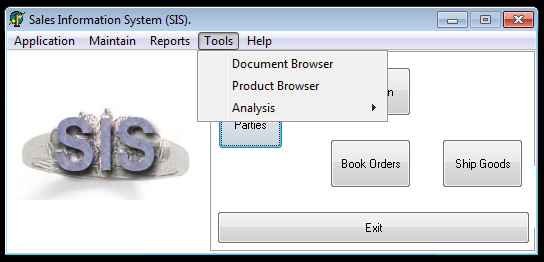
\includegraphics[width=0.4\textwidth]{./images/sis_lobby_tools.png}
  \caption{Lobby Tools menu}
  \label{fig:sis_lobby_tools}
\end{figure}

By clicking on \texttt{Document Browser} a window with the same name will open.

\begin{figure}[H]
  \centering
  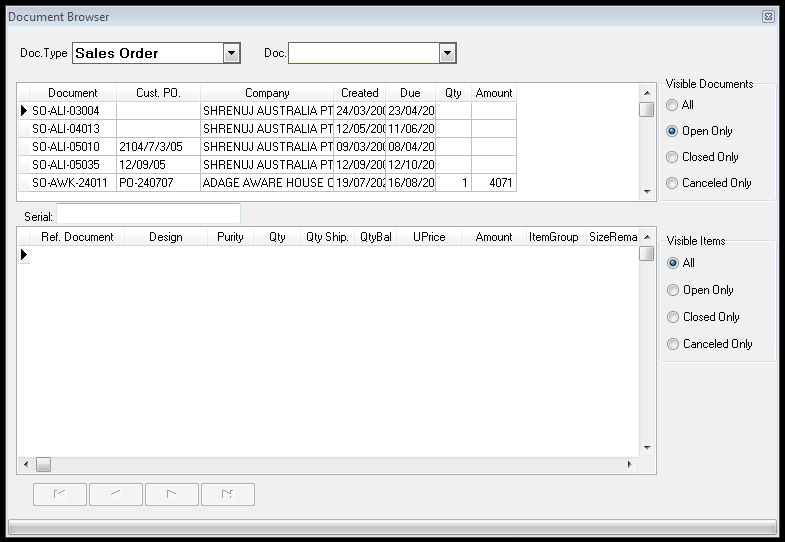
\includegraphics[width=0.4\textwidth]{./images/sis_lobby_tools_documentbrowser.png}
  \caption{Document Browser window}
  \label{fig:sis_lobby_tools_documentbrowser}
\end{figure}

It allows you to search through all kinds of \texttt{Documents} regardless of their type (\texttt{Sales Order}, etc).

By clicking on \texttt{Product Browser} the window \texttt{Product Prices} will open.

\begin{figure}[H]
  \centering
  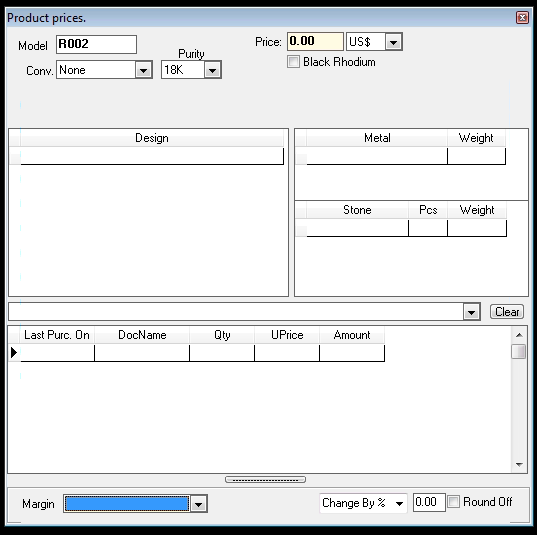
\includegraphics[width=0.4\textwidth]{./images/sis_lobby_tools_productprices.png}
  \caption{Product Prices window}
  \label{fig:sis_lobby_tools_productbrowser}
\end{figure}

It allows you to search through the \texttt{Product} by entering the \texttt{Model} name and selecting the \texttt{Design}.

By clicking on \texttt{Analysis} one more drop-down menu appeared.

\begin{figure}[H]
  \centering
  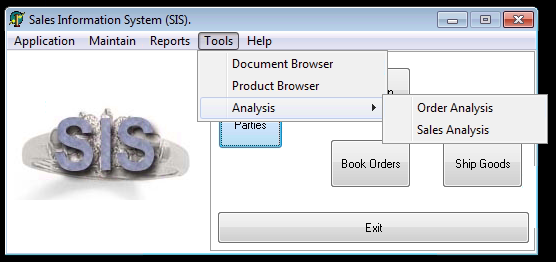
\includegraphics[width=0.4\textwidth]{./images/sis_lobby_tools_analysis.png}
  \caption{Analysis sub-menu under Tools}
  \label{fig:sis_lobby_tools_analysis}
\end{figure}

But by clicking on any of those two options \texttt{Order Analysis} and \texttt{Sales Analysis}, nothing happens.

\subsubsection*{Lobby Help}
On the toolbar, if you click on \texttt{Help} a drop-down menu appeared.

\begin{figure}[H]
  \centering
  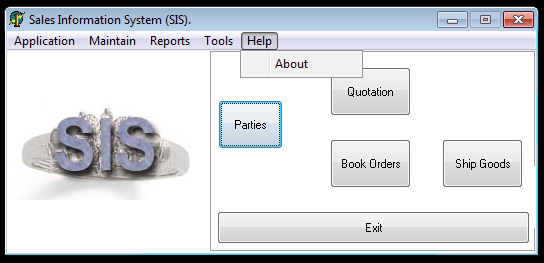
\includegraphics[width=0.4\textwidth]{./images/sis_lobby_help.png}
  \caption{Lobby Help menu}
  \label{fig:sis_lobby_help}
\end{figure}

The button \texttt{About} will open.  
This is useless.

